This project is about implementing a FM demodulator in VHDL, more precisely an incoherent demodulation. Figure \ref{fig:induction} illustrates the system and process.

\begin{figure}[h]
 \centering
 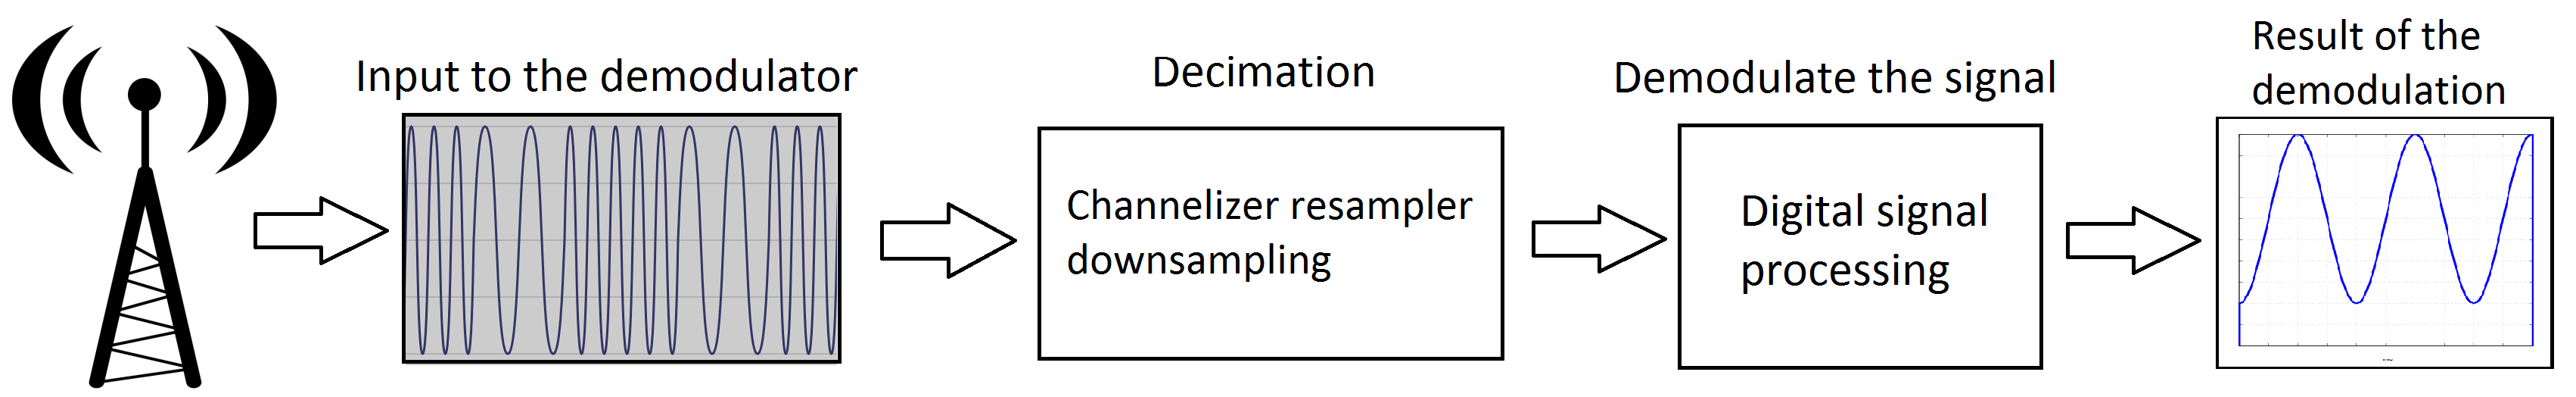
\includegraphics[scale=0.2]{images/induc.png}
 \caption{Demodulator process}
 \label{fig:induction}
\end{figure}

The input signal to the demodulator is a generated signal by Matlab. Matlab generates a text file with the coordinates of the input signal, which the simulation is able to read. Then the signal will be demodulated, which is the main goal for this project. The output signal of the demodulation will be write to another text file, so it can be plotted by Matlab for further investigating.